\documentclass[8pt,xcolor=table,aspectratio=169]{beamer}

\usepackage{graphicx}
\usepackage{caption}
\usepackage{subcaption}
\usepackage{transparent}
\usepackage{epstopdf} %converting to PDF
\usepackage{multicol} 
\usepackage{animate}[2017/05/18]

\usepackage{amsmath}
\usepackage{amssymb}
\usepackage{mathtools}
% \usepackage[utf8]{inputenc}
% \usepackage[T1]{fontenc}
% \usepackage[thinc]{esdiff}

% \usepackage{pdfx}
 
% \usepackage[utf8]{inputenc}
% \usepackage[T1]{fontenc}
\usepackage[table]{xcolor}    % loads also »colortbl« 
%  \usepackage{enumitem}
% \usepackage{ucltemplate}
\usepackage{color}

\usepackage{comment}

\usepackage{tabularx} % make width of table columns evenly distributed (see http://tex.stackexchange.com/questions/60601/evenly-distributing-column-widths)
% \newcolumntype{Y}{>{\centering\arraybackslash}X}

% make entire row bold or italic in table
\newcommand\setrow[1]{\gdef\rowmac{#1}#1\ignorespaces}
\newcommand\clearrow{\global\let\rowmac\relax}
\clearrow


\usepackage{amssymb}% http://ctan.org/pkg/amssymb
\usepackage{pifont}% http://ctan.org/pkg/pifont
\newcommand{\cmark}{\ding{51}}%
\newcommand{\xmark}{\ding{55}}%


%\usepackage{pgfgantt} % for grantt charts
\usepackage{rotating}
\usepackage[graphicx]{realboxes}
\usepackage[export]{adjustbox}
\usepackage{array}

\usepackage{rotating}
% \usepackage{tabularx, booktabs} % make width of table columns evenly distributed (see http://tex.stackexchange.com/questions/60601/evenly-distributing-column-widths)
% \newcolumntype{Y}{>{\centering\arraybackslash}X}

\DeclareMathOperator*{\argmin}{arg\,min}
\DeclareMathOperator*{\argmax}{arg\,max}

\usepackage{tikz}
\usetikzlibrary{bayesnet}
\usetikzlibrary{decorations}
\usetikzlibrary{decorations.pathreplacing}
\usetikzlibrary{arrows,positioning, shapes.symbols,shapes.callouts,patterns,shapes,chains,calc,backgrounds,fadings}

% \definecolor{parCol}{rgb}{0.1, 0.1, 1}
% \definecolor{stCol}{rgb}{0.1, 0.6, 0.1}
% \definecolor{bothCol}{rgb}{0, 0.5, 0.5}

\definecolor{parCol}{rgb}{0, 0, 0}
\definecolor{stCol}{rgb}{0, 0, 0}
\definecolor{bothCol}{rgb}{0, 0, 0}
\definecolor{blue3}{HTML}{86B7FC} % med blue
\definecolor{blue1}{HTML}{B5F1FF} % light blue
\definecolor{blue2}{HTML}{E0F9FF} % very light blue

\newcolumntype{C}[1]{>{\centering\let\newline\\\arraybackslash\hspace{0pt}}m{#1}}

\setlength{\tabcolsep}{0.2em}

 
 %% OVERVIEW OF WORK SO FAR %%
 
%Information to be included in the title page:
\title{Bayesian Image Reconsturuction using Deep Generative Models}
\author[Raz]{
R\u{a}zvan V. Marinescu\vspace{1em}}

\institute{\small{Massachusetts Institute of Technology}

% \vspace{0em}
% \small{Centre for Medical Image Computing, University College London, UK}
}

\date{}

% logo of my university
\titlegraphic{
   \begin{figure}
%    \begin{subfigure}{0.32\textwidth}
%    \hspace{2em}
%    
\includegraphics[height=1.0cm]{ucl_logo}
%    \end{subfigure}
   \begin{subfigure}{0.32\textwidth}
   \centering
   
\includegraphics[height=1.0cm]{MIT_logo.png} 
   \end{subfigure}
%    \begin{subfigure}{0.32\textwidth}
%    \centering
%    
\includegraphics[height=1.0cm]{pondLogo.png} 
%    \end{subfigure}
   \end{figure}
   
%    \tiny{Slides available online: https://people.csail.mit.edu/razvan/talk/martinos2019/pres.pdf}
}

\setbeamercolor{frametitle}{fg=black}
\setbeamercolor{author in head/foot}{fg=black, bg=white} 
\setbeamercolor{institute in head/foot}{fg=black, bg=white} 
\setbeamercolor{title in head/foot}{fg=black, bg=white}
\setbeamercolor{date in head/foot}{fg=black, bg=white}

\setbeamersize{text margin left=10pt,text margin right=10pt}
% \setbeamertemplate{frametitle}{
%     \vspace{0.9em}
%     \insertframetitle
% %     \vspace{-3em}
% }
\setbeamertemplate{frametitle}{%
    \vspace{0.5em}
    \usebeamerfont{frametitle}\insertframetitle%
    \vphantom{g}% To avoid fluctuations per frame
    %\hrule% Uncomment to see desired effect, without a full-width hrule
    \par% <-- added
    \hspace*{-\dimexpr0.5\paperwidth-0.5\textwidth}% <-- calculation of left margin width
    \rule[0.5\baselineskip]{\paperwidth}{0.4pt}%
}

\setbeamertemplate{footline}
{
  \vspace{-3em}
  \leavevmode%
   \rule{\paperwidth}{0.3pt}
  \hbox{%
  \begin{beamercolorbox}[wd=.2\paperwidth,ht=2.25ex,dp=1ex,center]{author in head/foot}%
    \usebeamerfont{author in head/foot}Razvan V. Marinescu
  \end{beamercolorbox}%
  \begin{beamercolorbox}[wd=.2\paperwidth,ht=2.25ex,dp=1ex,center]{institute in head/foot}%
    \usebeamerfont{institute in head/foot}razvan@csail.mit.edu
  \end{beamercolorbox}%
  \begin{beamercolorbox}[wd=.3\paperwidth,ht=2.25ex,dp=1ex,center]{institute in head/foot}%
    \usebeamerfont{institute in head/foot}http://razvan.csail.mit.edu
  \end{beamercolorbox}%
  \begin{beamercolorbox}[wd=.2\paperwidth,ht=2.25ex,dp=1ex,center]{title in head/foot}%
    \usebeamerfont{title in head/foot}\insertsection
  \end{beamercolorbox}%
  \begin{beamercolorbox}[wd=.10\paperwidth,ht=2.25ex,dp=1ex,right]{date in head/foot}%
    \usebeamerfont{date in head/foot}\insertshortdate{}\hspace*{2em}
    \insertframenumber{} / \inserttotalframenumber\hspace*{2ex}
  \end{beamercolorbox}}%
  \vskip0pt%
}

% \usepackage{beamerthemesplit}

\newcommand{\backupbegin}{
   \newcounter{finalframe}
   \setcounter{finalframe}{\value{framenumber}}
}
\newcommand{\backupend}{
   \setcounter{framenumber}{\value{finalframe}}
}


\makeatletter
\long\def\beamer@author[#1]#2{%
  \def\and{\tabularnewline}
  \def\insertauthor{\def\inst{\beamer@insttitle}\def\and{\tabularnewline}%
  \begin{tabular}{rl}#2\end{tabular}}%
  \def\beamer@shortauthor{#1}%
  \ifbeamer@autopdfinfo%
    \def\beamer@andstripped{}%
    \beamer@stripands#1 \and\relax
    {\let\inst=\@gobble\let\thanks=\@gobble\def\and{, }\hypersetup{pdfauthor={\beamer@andstripped}}}
  \fi%
}
\makeatother
\beamertemplatenavigationsymbolsempty
\setbeamertemplate{caption}[numbered]
\setbeamercolor{caption name}{fg=black}
\setbeamercolor{itemize item}{fg=black}
\setbeamercolor{itemize subitem}{fg=black}
\setbeamercolor{enumerate item}{fg=black}
\setbeamercolor{enumerate subitem}{fg=black}
\setbeamertemplate{enumerate item}[default]
\setbeamertemplate{enumerate subitem}[default]

\makeatletter
\let\@@magyar@captionfix\relax
\makeatother
\begin{document}
 
\section{Introduction}

\frame{\titlepage}
 
\setbeamerfont{frametitle}{size=\large}

\newcommand{\upgradeReportLoc}{../../upgrade_report}
\newcommand{\epsrcPresLoc}{\upgradeReportLoc/epsrcPres}
\newcommand{\jointModellingDiseaseLoc}{../../jointModellingDisease}
\newcommand{\pcaLongPaperLoc}{../../PCA_long_paper}
\newcommand{\voxFld}{../../voxelwiseDPM}
\newcommand{\tadpoleFld}{../../tadpole}
\newcommand{\diffEqModelFld}{../../diffEqModel}

\newcommand{\outFolder}{../overview/modelDiagram}
\newcommand{\lw}{0.5mm}

\newcommand{\yes}{{\LARGE \textcolor{green!50!black}{\checkmark} \par}}
\newcommand{\no}{{\LARGE \textcolor{red}{\xmark} \par}}



\newcommand*{\pcaLongFigs}{\pcaLongPaperLoc/figures}


% \includeonlyframes{1-20}
%\includeonlyframes{current}



\newcommand{\ovHeight}{2cm}
\newcommand{\vo}{\vspace{1em}}
\newcommand{\vt}{\vspace{2em}}
\newcommand{\vth}{\vspace{3em}}


% % TODO continue with overview, move into commands
\newcommand{\ovEBM}{
\begin{subfigure}{0.47\textwidth}
\centering
1. Modelled progression of PCA and tAD\\
(using existing methods)
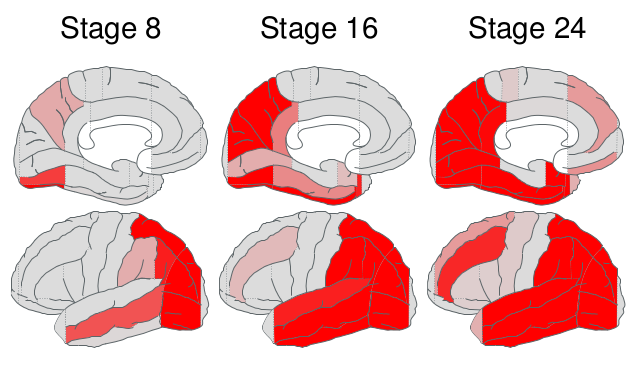
\includegraphics[height=\ovHeight]{ebm_thumb.png}
\end{subfigure}
}

\newcommand{\ovVWDPM}{
\begin{subfigure}{0.47\textwidth}
\centering
% \vspace{2.8em}
2. Developed Novel Spatio-temporal Model \\ (DIVE)\\
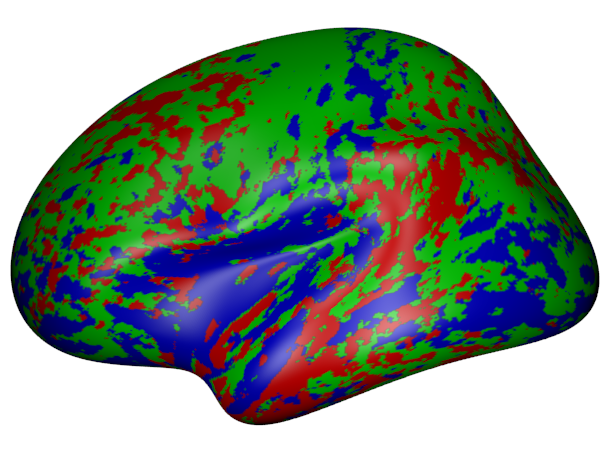
\includegraphics[height=\ovHeight]{\upgradeReportLoc/images/vwdpm/blend14_adniThavgFWHM0InithistCl3Pr0Ra1_VWDPMStd.png}
\end{subfigure}
}


\newcommand{\ovDKT}{
\begin{subfigure}{0.47\textwidth}
\centering
\vspace{2em}
3. Developed Novel Transfer Learning \\ method (DKT) \\
\vspace{0.5em}
\includegraphics[height=2.2cm]{\jointModellingDiseaseLoc/paper/figures/disease_knowledge_transfer.pdf}
\end{subfigure}
}


\newcommand{\ovTadpole}{
\begin{subfigure}{0.47\textwidth}
\centering
\vspace{-2em}
4. Organised TADPOLE Competition\\
\vspace{1em}
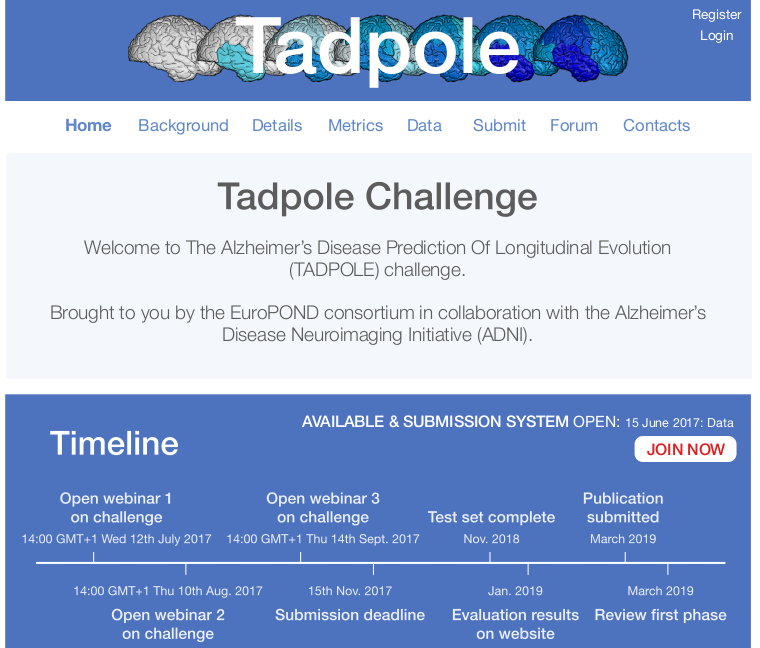
\includegraphics[height=1.2cm,valign=t]{\upgradeReportLoc/epsrcPres/tadpole} 
\end{subfigure}
}

\newcommand{\ovPainter}{
\begin{subfigure}{\textwidth}
\centering
\vspace{0.5em}
5. Created BrainPainter software\\
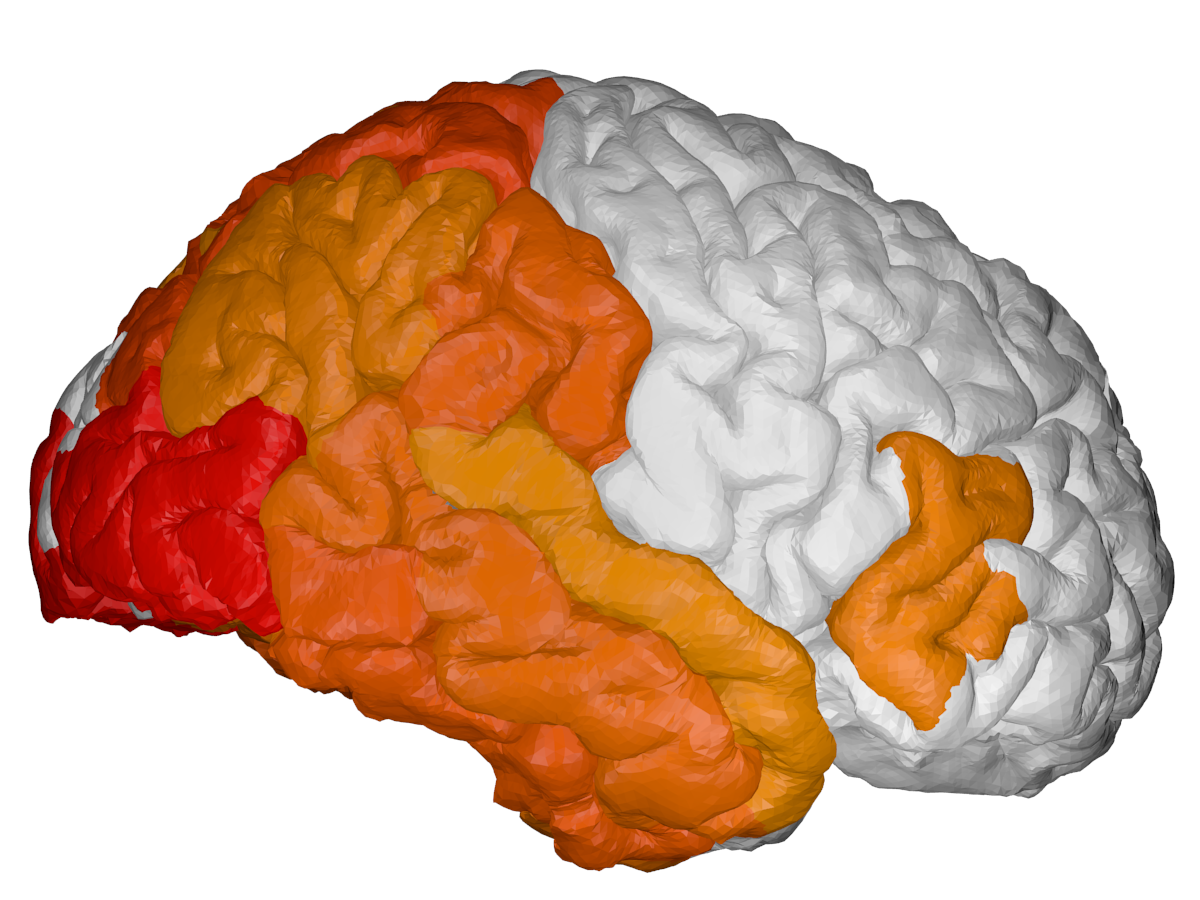
\includegraphics[height=1.5cm]{cortical-front_1}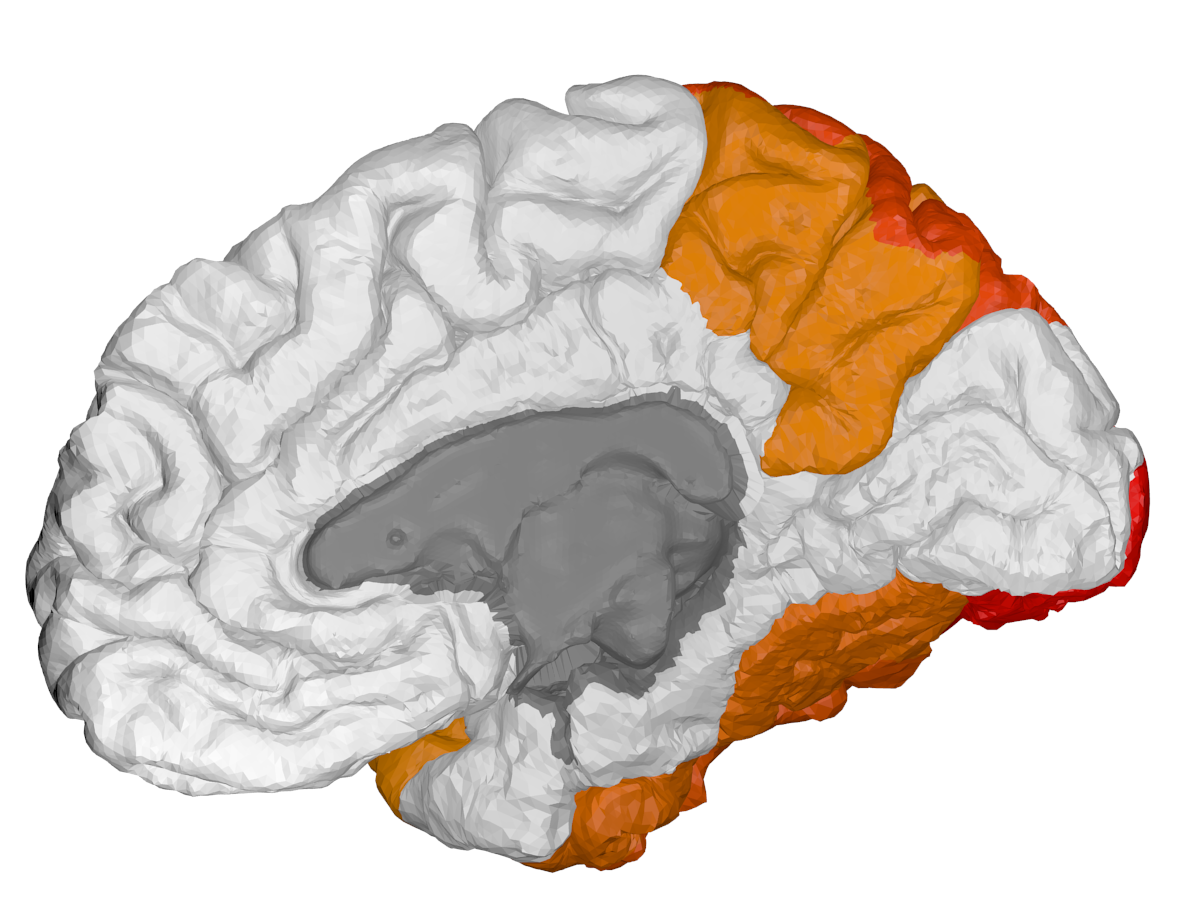
\includegraphics[height=1.5cm]{cortical-back_1}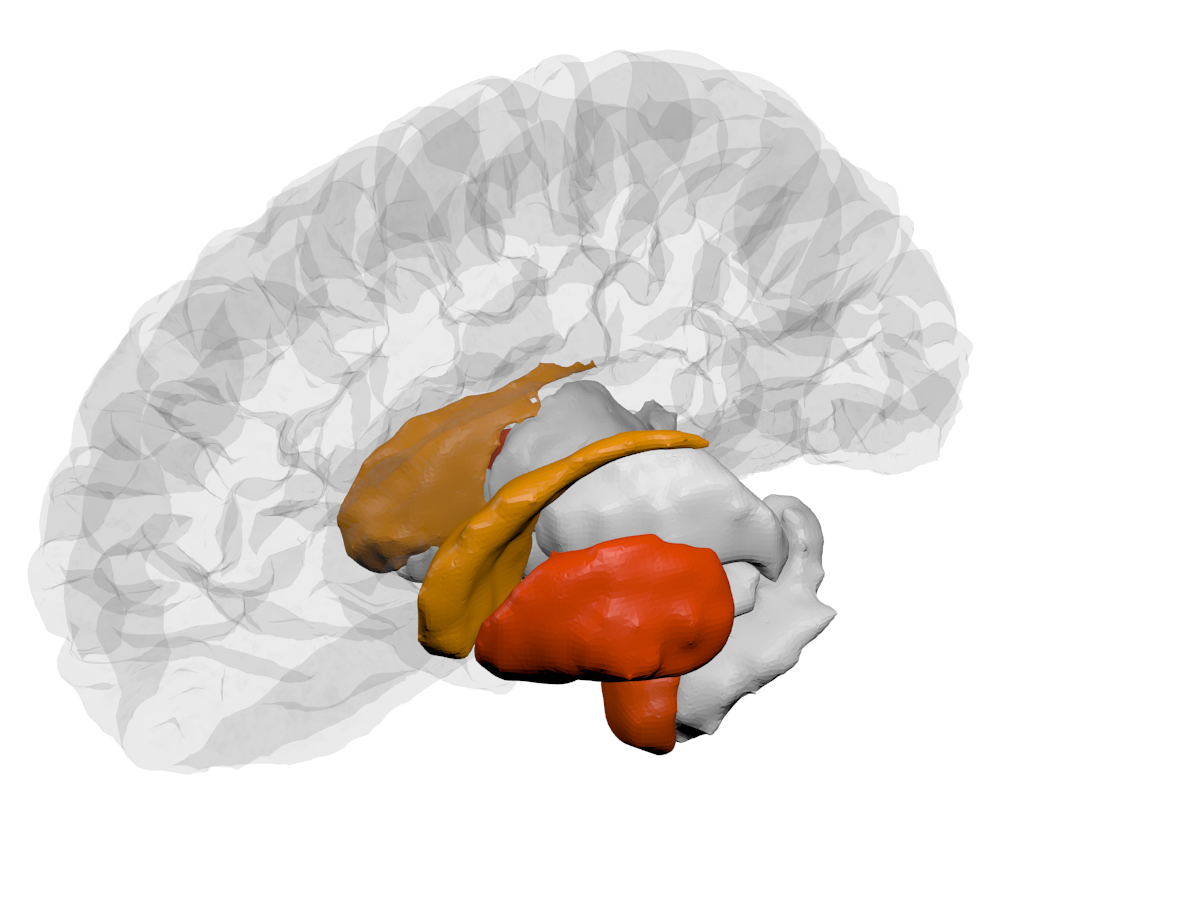
\includegraphics[height=1.5cm]{subcortical_1}
\end{subfigure}
}


\definecolor{light-gray}{gray}{0.6}


\newcommand{\inc}[1]{\includegraphics[width=\columnwidth, trim=4 4 4 4, clip]{#1}}
\newcommand{\incw}[2]{\includegraphics[width=#2\columnwidth, trim=4 4 4 4, clip]{#1}}
\newcommand{\inch}[2]{\includegraphics[height=#2, trim=4 4 4 4, clip]{#1}}












\newcommand{\diagfld}{brgm_diagram}
\newcommand{\fstikz}[1]{\footnotesize{#1}}

\newcommand{\dgs}{0.85}

\newcommand{\brgmprev}{
\begin{tikzpicture}[scale=\dgs, every node/.style={scale=\dgs}]

\def\rightimgX{4.5}

%top image center
\node (cxr_img) at (1, 3.5) {
\includegraphics[width=2cm]{\diagfld/brain_target}};
\node (cxr_text) at (1,4.75) {\footnotesize{Low Res.}};

%top image left
\node (blur_img) at (\rightimgX, 3.5) {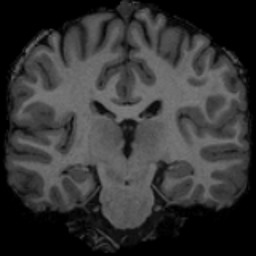
\includegraphics[width=2cm]{\diagfld/brain_clean}};
\node (blur_text) at (\rightimgX,4.75) {\footnotesize{High Res.}};

%top image center
\node (cxr_img) at (1, 1) {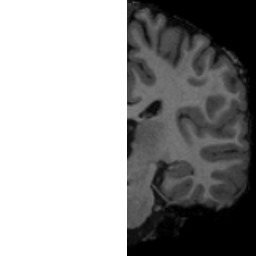
\includegraphics[width=2cm,frame]{\diagfld/brain_inpaint}};
%top image left
\node (blur_img) at (\rightimgX, 1) {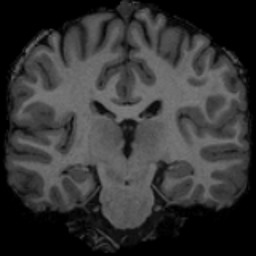
\includegraphics[width=2cm]{\diagfld/brain_clean}};

\node (left_img_top_out) at (2,3.5) {};
\node (right_img_top_in) at (\rightimgX - 1, 3.5) {};

\draw[->, thick]
(left_img_top_out)
to
(right_img_top_in) ;


\node (left_img_top_out_2) at (2,1) {};
\node (right_img_top_in_2) at (\rightimgX - 1, 1) {};

\draw[->, thick]
(left_img_top_out_2)
to
(right_img_top_in_2) ;


\node (left_img_top_in) at (2,2.5) {};
\node (right_img_top_out) at (\rightimgX - 1, 2.5) {};

\node (rng_text) at (2.75,3.75) {$f_1^{-1}$};
\node (rng_text) at (2.75,3.25) {\fstikz{Learned}};
\node (rng_text) at (2.75,3) {\fstikz{Inverse}};
\node (rng_text) at (2.75,2.75) {\fstikz{Corruption}};

\node (rng_text) at (2.75,1.25) {$f_2^{-1}$};

\end{tikzpicture}
}

\newcommand{\brgmours}{
\begin{tikzpicture}[scale=\dgs, every node/.style={scale=\dgs}]

\def\rightimgX{4.5}

%Top left
\filldraw[fill=gray!50!white, draw=black, label={Latent}] (-2,2.5) rectangle (-1.5,4.5);
\node (rng_text) at (-1.75,4.75) {\footnotesize{Latent}};
\node (rng_text) at (-1.75,3.5) {$w$};

%top image center
\node (cxr_img) at (1, 3.5) {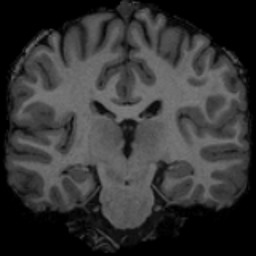
\includegraphics[width=2cm]{\diagfld/brain_clean}};
\node (cxr_text) at (1,4.75) {\footnotesize{High Res.}};

%top image right
\node (blur_img) at (\rightimgX, 3.5) {
\includegraphics[width=2cm]{\diagfld/brain_target}};
\node (blur_text) at (\rightimgX,4.75) {\footnotesize{Low Res.}};

\node (blur_img) at (\rightimgX+2.3, 3.5) {
\includegraphics[width=2cm]{\diagfld/brain_target}};
\node (blur_text) at (\rightimgX+2.3,4.75) {\footnotesize{Input}};

\draw[decoration={brace,mirror,raise=5pt},decorate]
  (4.5,2.5) -- node[below=6pt] {loss} (6.8,2.5);


\node (rng_top_out) at (-1.5,3.5) {};
\node (center_img_left_in) at (0, 3.5) {};

\draw[->, thick]
(rng_top_out)
to
(center_img_left_in) ;
\node (left_img_top_out) at (2,3.5) {};
\node (right_img_top_in) at (\rightimgX - 1, 3.5) {};

\draw[->, thick]
(left_img_top_out)
to
(right_img_top_in) ;

\node (left_img_top_in) at (2,2.5) {};
\node (right_img_top_out) at (\rightimgX - 1, 2.5) {};

% \draw[->, dashed, blue, thick]
% (right_img_top_out)
% to [in=-60, out=-120]
% (left_img_top_in) ;


\node (left_img_bot_out) at (0,2.5) {};
\node (rng_bot_out) at (-1.5, 2.5) {};
%\draw[->, dashed, red, thick]
%(rng_bot_out)
%to [in=-120, out=-60]
%(left_img_bot_out);

\node (rng_text) at (-0.75,3.75) {$G(w)$};
\node (rng_text) at (-0.75,3.25) {\fstikz{Image}};
\node (rng_text) at (-0.75,3) {\fstikz{Generation}};

\node (rng_text) at (2.75,3.75) {$f_1$};
\node (rng_text) at (2.75,3.25) {\fstikz{Known}};
\node (rng_text) at (2.75,3) {\fstikz{Corruption}};


\node (left_img_center_out) at (1,2.5) {};
\node (right_bot_out_extra) at (3.9 - 1, 1) {};
\draw[->, thick]
(left_img_center_out)
to [in=90, out=-90]
(1,1) 
to [out=0, in=180]
(right_bot_out_extra);

\node (right_bot_out_extra_2) at (3.9 - 1, 0.5) {};
\draw[->, thick]
(left_img_center_out)
to [in=90, out=-90]
(1,0.5) 
to [out=0, in=180]
(right_bot_out_extra_2);


\node (rng_text) at (1.75,1.25) {$f_2$};
\node (rng_text) at (1.75,0.75) {$f_3$};
\node (rng_text) at (1.75,0.25) {$\vdots$};


\node (blur_img) at (3.5+0.5, 0.5) {
\includegraphics[width=1cm]{\diagfld/brain_kspace.png}};
\node (blur_img) at (3.5, 1.0) {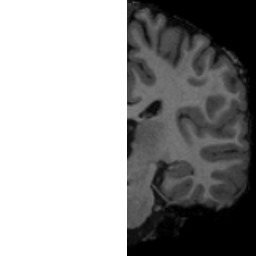
\includegraphics[width=1cm,frame]{\diagfld/brain_inpaint}};

\end{tikzpicture}
}


\newcommand{\brgmoursshortloss}{
\begin{tikzpicture}[scale=\dgs, every node/.style={scale=\dgs}]

\def\rightimgX{4.5}

%Top left
\filldraw[fill=gray!50!white, draw=black, label={Latent}] (-2,2.5) rectangle (-1.5,4.5);
\node (rng_text) at (-1.75,4.75) {\footnotesize{Latent}};
\node (rng_text) at (-1.75,3.5) {$w$};

%top image center
\node (cxr_img) at (1, 3.5) {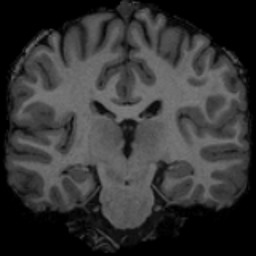
\includegraphics[width=2cm]{\diagfld/brain_clean}};
\node (cxr_text) at (1,4.75) {\footnotesize{High Res.}};

%top image right
\node (blur_img) at (\rightimgX, 3.5) {
\includegraphics[width=2cm]{\diagfld/brain_target}};
\node (blur_text) at (\rightimgX,4.75) {\footnotesize{Low Res.}};

\node (blur_img) at (\rightimgX+2.3, 3.5) {
\includegraphics[width=2cm]{\diagfld/brain_target}};
\node (blur_text) at (\rightimgX+2.3,4.75) {\footnotesize{Input}};

\draw[decoration={brace,mirror,raise=5pt},decorate]
  (4.5,2.5) -- node[below=6pt] {loss} (6.8,2.5);


\node (rng_top_out) at (-1.5,3.5) {};
\node (center_img_left_in) at (0, 3.5) {};

\draw[->, thick]
(rng_top_out)
to
(center_img_left_in) ;
\node (left_img_top_out) at (2,3.5) {};
\node (right_img_top_in) at (\rightimgX - 1, 3.5) {};

\draw[->, thick]
(left_img_top_out)
to
(right_img_top_in) ;

\node (left_img_top_in) at (2,2.5) {};
\node (right_img_top_out) at (\rightimgX - 1, 2.5) {};

% \draw[->, dashed, blue, thick]
% (right_img_top_out)
% to [in=-60, out=-120]
% (left_img_top_in) ;


\node (left_img_bot_out) at (0,2.5) {};
\node (rng_bot_out) at (-1.5, 2.5) {};
%\draw[->, dashed, red, thick]
%(rng_bot_out)
%to [in=-120, out=-60]
%(left_img_bot_out);

\node (rng_text) at (-0.75,3.75) {$G(w)$};
\node (rng_text) at (-0.75,3.25) {\fstikz{Image}};
\node (rng_text) at (-0.75,3) {\fstikz{Generation}};

\node (rng_text) at (2.75,3.75) {$f_1$};
\node (rng_text) at (2.75,3.25) {\fstikz{Known}};
\node (rng_text) at (2.75,3) {\fstikz{Corruption}};


%\node (left_img_center_out) at (1,2.5) {};
%\node (right_bot_out_extra) at (3.9 - 1, 1) {};
%\draw[->, thick]
%(left_img_center_out)
%to [in=90, out=-90]
%(1,1) 
%to [out=0, in=180]
%(right_bot_out_extra);
%
%\node (right_bot_out_extra_2) at (3.9 - 1, 0.5) {};
%\draw[->, thick]
%(left_img_center_out)
%to [in=90, out=-90]
%(1,0.5) 
%to [out=0, in=180]
%(right_bot_out_extra_2);


%\node (rng_text) at (1.75,1.25) {$f_2$};
%\node (rng_text) at (1.75,0.75) {$f_3$};
%\node (rng_text) at (1.75,0.25) {$\vdots$};
%
%
%\node (blur_img) at (3.5+0.5, 0.5) {
\includegraphics[width=1cm]{\diagfld/brain_kspace.png}};
%\node (blur_img) at (3.5, 1.0) {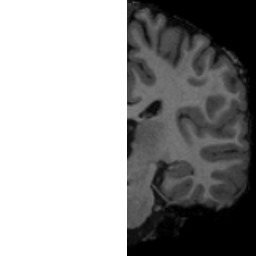
\includegraphics[width=1cm,frame]{\diagfld/brain_inpaint}};

\end{tikzpicture}
}


\newcommand{\brgmoursshort}{
\begin{tikzpicture}[scale=0.75, every node/.style={scale=0.75}]

\def\rightimgX{4.5}

%Top left
\filldraw[fill=gray!50!white, draw=black, label={Latent}] (-2,2.5) rectangle (-1.5,4.5);
\node (rng_text) at (-1.75,4.75) {\footnotesize{Latent}};
\node (rng_text) at (-1.75,3.5) {$w$};

%top image center
\node (cxr_img) at (1, 3.5) {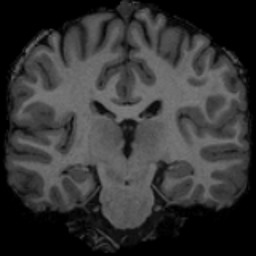
\includegraphics[width=2cm]{\diagfld/brain_clean}};
\node (cxr_text) at (1,4.75) {\footnotesize{High Res.}};

%top image right
\node (blur_img) at (\rightimgX, 3.5) {
\includegraphics[width=2cm]{\diagfld/brain_target}};
\node (blur_text) at (\rightimgX,4.75) {\footnotesize{Low Res.}};

\node (rng_top_out) at (-1.5,3.5) {};
\node (center_img_left_in) at (0, 3.5) {};

\draw[->, thick]
(rng_top_out)
to
(center_img_left_in) ;

\node (left_img_top_out) at (2,3.5) {};
\node (right_img_top_in) at (\rightimgX - 1, 3.5) {};

\draw[->, thick]
(left_img_top_out)
to
(right_img_top_in) ;

\node (left_img_top_in) at (2,2.5) {};
\node (right_img_top_out) at (\rightimgX - 1, 2.5) {};

\node (left_img_bot_out) at (0,2.5) {};
\node (rng_bot_out) at (-1.5, 2.5) {};


% \node (rng_text) at (-0.75,3.75) {$G(w)$};
\node (rng_text) at (-0.75,3.25) {\fstikz{Image}};
\node (rng_text) at (-0.75,3) {\fstikz{Generation}};

% \node (rng_text) at (2.75,3.75) {$f_1$};
\node (rng_text) at (2.75,3.25) {\fstikz{Known}};
\node (rng_text) at (2.75,3) {\fstikz{Corruption}};

\end{tikzpicture}
}





\section{Bayesian Image Reconstruction}


\newcommand{\mrirecon}{
\begin{tikzpicture}[scale=0.75, every node/.style={scale=0.75}]

\def\rightimgX{4.2}

%Top left
% \filldraw[fill=gray!50!white, draw=black, label={Latent}] (-2,2.5) rectangle (-1.5,4.5);
% \node (rng_text) at (-1.75,4.75) {\footnotesize{Latent}};
% \node (rng_text) at (-1.75,3.5) {$w$};

%top image center
\node (cxr_img) at (\rightimgX, 3.5) {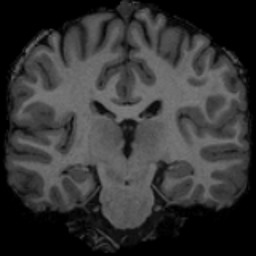
\includegraphics[width=2cm]{\diagfld/brain_clean}};
% \node (cxr_text) at (1,4.75) {\footnotesize{High Res.}};

%top image right
\node (blur_img) at (1, 3.5) {
\includegraphics[width=2cm]{\diagfld/brain_target}};
% \node (blur_text) at (\rightimgX,4.75) {\footnotesize{Low Res.}};

% \node (rng_top_out) at (-1.5,3.5) {};
% \node (center_img_left_in) at (0, 3.5) {};

% \draw[->, thick]
% (rng_top_out)
% to
% (center_img_left_in) ;

\node (left_img_top_out) at (2,3.5) {};
\node (right_img_top_in) at (\rightimgX - 1, 3.5) {};

\draw[->, thick]
(left_img_top_out)
to
(right_img_top_in) ;

% \node (left_img_top_in) at (2,2.5) {};
% \node (right_img_top_out) at (\rightimgX - 1, 2.5) {};

% \node (left_img_bot_out) at (0,2.5) {};
% \node (rng_bot_out) at (-1.5, 2.5) {};


% \node (rng_text) at (-0.75,3.75) {$G(w)$};
% \node (rng_text) at (-0.75,3.25) {\fstikz{Image}};
% \node (rng_text) at (-0.75,3) {\fstikz{Generation}};

% \node (rng_text) at (2.75,3.75) {$f_1$};
% \node (rng_text) at (2.75,3.25) {\fstikz{Known}};
% \node (rng_text) at (2.75,3) {\fstikz{Corruption}};

\end{tikzpicture}
}


\newcommand{\brgmfull}{
\begin{tikzpicture}[scale=0.75, every node/.style={scale=0.75}]

\def\rightimgX{4.2}

%Top left
% \filldraw[fill=gray!50!white, draw=black, label={Latent}] (-2,2.5) rectangle (-1.5,4.5);
% \node (rng_text) at (-1.75,4.75) {\footnotesize{Latent}};
% \node (rng_text) at (-1.75,3.5) {$w$};

%top image center
\node (cxr_img) at (\rightimgX, 3.5) {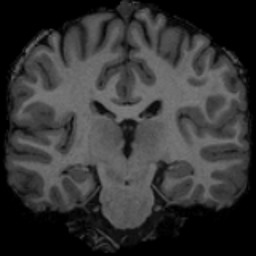
\includegraphics[width=2cm]{\diagfld/brain_clean}};
% \node (cxr_text) at (1,4.75) {\footnotesize{High Res.}};

%top image right
\node (blur_img) at (1, 3.5) {
\includegraphics[width=2cm]{\diagfld/brain_target}};
% \node (blur_text) at (\rightimgX,4.75) {\footnotesize{Low Res.}};

% \node (rng_top_out) at (-1.5,3.5) {};
% \node (center_img_left_in) at (0, 3.5) {};

% \draw[->, thick]
% (rng_top_out)
% to
% (center_img_left_in) ;

\node (left_img_top_out) at (2,3.5) {};
\node (right_img_top_in) at (\rightimgX - 1, 3.5) {};

\draw[->, thick]
(left_img_top_out)
to
(right_img_top_in) ;

 \node (left_img_top_in) at (2,2.5) {};
 \node (right_img_top_out) at (\rightimgX - 1, 2.5) {};

% \node (left_img_bot_out) at (0,2.5) {};
 \node (rng_bot_out) at (-1.5, 2.5) {};


 \node (rng_text) at (-0.75,3.75) {$G(w)$};
 \node (rng_text) at (-0.75,3.25) {\fstikz{Image}};
 \node (rng_text) at (-0.75,3) {\fstikz{Generation}};

% \node (rng_text) at (2.75,3.75) {$f_1$};
 \node (rng_text) at (2.75,3.25) {\fstikz{Known}};
 \node (rng_text) at (2.75,3) {\fstikz{Corruption}};

\end{tikzpicture}
}

\begin{frame}{Aim: image reconstruction using *pre-trained* generator models}

\begin{columns}
 \begin{column}{0.5\textwidth}
  
  \begin{itemize}
   \item Adapt the state-of-the-art StyleGAN2 for medical image reconstruction

%    \vspace{2em}
   
%    \item Vision: bring this technology to medicine
  \end{itemize}
  
 \vspace{1em}
 
%   \begin{column}{0.5\textwidth}
%   \centering
% %   MRI generation\\
% %   \incw{\diagfld/brain_clean}{0.4}
% 
%   \end{column}
  \begin{column}{\textwidth}
  \centering
  MRI reconstruction\\
  \mrirecon
  
  \end{column}
  
 \end{column} 
 
 \begin{column}{0.5\textwidth}
 \centering
 StyleGAN2 (Karras et al, 2019)
 \incw{stylegan}{0.8} 
 \end{column}

\end{columns}



\end{frame}

\begin{frame}{Current image reconstruction methods have several limitations}


\begin{columns}
 \begin{column}{0.5\textwidth}

 \begin{itemize}
 \item Require large computational resources and data
 
 \vt
 
 \item Are specific to particular corruption tasks
 
 \vt 
 
 \item Cannot deal with distribution shifts:
 \begin{itemize}
   \item in inputs: e.g. older populations
   \item in corruption type: e.g. change in blur kernel
 \end{itemize}
 
  
 \end{itemize}

 \end{column}

 \begin{column}{0.5\textwidth}
  \centering
%\incw{task-specific}{0.8}
 \brgmprev  
  
 \end{column}
\end{columns} 

 
\end{frame}



\begin{frame}{Limitation 1: State-of-the-art DL methods have large computational requirements}

\begin{itemize}
\item Requirements = Computation Time + Advanced Hardware + Large Datasets

\vo 

\item Most computation now runs on clouds\\ 
%  \begin{itemize}
%  \item Large computational resources
%  \item Large datasets
%  \item Long time to converge
% \end{itemize}

 \incw{datacenter}{0.5}

\vo

 \item Currently few labs/companies have the resources to train state-of-the-art models
 \begin{itemize}
  \item StyleGAN2: 9 days on 4 GPUs
  \item GPT-3: 355 years on single GPU
 \end{itemize}

 
\vo


\vo
 \item Solutions moving forward:
 \begin{itemize}
\item Adapting previously-trained models
\item Combine smaller models into larger ones
\end{itemize}
\end{itemize}

 
\end{frame}

\begin{frame}{Limitation 2: Distribution shifts require model re-training}


\begin{itemize}
 \item Distribution shifts happen all the time:
 \begin{itemize}
 \item Changes in hospital scanners, protocols, software upgrades
 \item Can be continuous: population getting older due to better healthcare
\end{itemize}

\vt
 \item Shifts can result in combinatorial effects in number of re-training instances!

\vt
 
 \item Compositionality is one potential solution
 
\end{itemize}
% \vspace{1em}

\begin{center}
\incw{compositionality}{1}
\end{center}
 
\end{frame}

\begin{frame}{Recent models can perform image reconstruction using \textbf{pre-trained} generative models}
 

 
\begin{columns}[t]
 \begin{column}{0.6\textwidth}
\centering
Image2StyleGAN++ (Abdal, 2020)\\
\inch{image2stylegan}{3cm}
 \end{column}

 \begin{column}{0.3\textwidth}
  \centering
  PULSE (Menon, Damian et al, 2020)\\
\inch{pulse}{3cm}
 
 \end{column}
\end{columns} 

\vspace{2em}

\begin{itemize}
 \item Don't use an embedder network, so can generalise beyond the training data
 \item However, they are specific to a particular corruption task (either in-painting or super-resolution)
 \item Cannot characterize \textbf{uncertainty} and recover \textbf{multiple solutions}
 \item We will aim to construct a Bayesian formulation that can fully characterize the posterior over all potential solutions
\end{itemize}


 
 
\end{frame}



% \begin{frame}{Limitation 3: Models are anti-causal}
% 
% 
% \begin{itemize}
%  \item Existing model don't follow the data-generation process
% \begin{itemize}
%    \item Discriminative modelling easier than generative
% \end{itemize}
% 
%  \vo
%  
%   
%  \vo 
%  
%  \item Causal modelling is the \textbf{right solution} to deal with distribution shifts
%  
%  \vo
%  
% %  \begin{itemize}
% %  \item Both for inputs and intermediary variables
% % \end{itemize}
% \end{itemize}
% 
% 
% \begin{center}
% \incw{causality}{0.8}
% \end{center}
%  
% \end{frame}


\begin{frame}{Method: We perform image reconstruction by combining two models\\
% \begin{itemize}
\ \ \ \ \ \  1. a pre-trained generator G (StyleGAN2)\\
\ \ \ \ \ \  2. a known forward corruption model $f_1$
% \end{itemize}
}



\begin{columns}[t]
 \begin{column}{0.6\textwidth}
\centering
 
\begin{overprint}
 %\onslide<1> \incw{brgm_diagram_loss}{1}
 %\onslide<2-> \incw{brgm_diagram_all}{1}
 
 \onslide<1> \brgmoursshortloss 
 \onslide<2-> \brgmours

\end{overprint} 
 \onslide<3> Ours (Marinescu et al, arXiv, 2020)
 \end{column}

 \begin{column}{0.3\textwidth}
  \centering

 %\onslide<3> \incw{task-specific}{1}
 \onslide<3> \brgmprev
 \onslide<3> Previous

 
 \end{column}
\end{columns} 
 


 
\end{frame}

\newcommand{\ci}[1]{\circ{#1}}
\newcommand{\wplus}{$\mathcal{W}^{+}$ }
\newcommand{\loss}{\mathcal{L}}

\newcommand{\bit}[1]{\begin{itemize} 
\item #1
\end{itemize}}

\begin{frame}{Reconstructed image is given by computing the Bayesian maximum a-posteriori (MAP) estimate\\
}



\begin{itemize}
 \item We optimise:
$$ w^* = \argmax_w p(w)p(I|w)$$

\item For uninformative prior $p(w)$ and Gaussian noise model (pixelwise independent), we get:

$$ w^* = \argmin_w || I - f \circ G (w) ||_2^2$$

\item This can be optimised with SGD

\item Once we get $w^*$, the the reconstructed image is $G(w^*)$

\end{itemize}

\begin{center}
\vt
%\incw{brgm_diagram_loss}{0.6}
\brgmoursshortloss
\end{center}
 
\end{frame}
% 

\newcommand{\txc}[1]{\mathbin{\textcolor{red}{#1}}}
\newcommand{\szb}{0.8}
\begin{frame}{Good reconstructions require further modifications}

\begin{columns}

\begin{column}{0.5\textwidth}
\begin{itemize}
  \item We started from the original StyleGAN2 inversion
 
 \vo
 
 \onslide<2-> \item Yet the reconstruction was not good $\to$ required several changes
\begin{overprint}
\onslide<3> \bit{remove noise layers}
\onslide<4> \bit{optimize latents at all resolutions}
\onslide<5> \bit{add pixelwise loss}
\onslide<6> \bit{gaussian prior on latents}
\onslide<7> \bit{force latents to be colinear}
\onslide<8> \bit{Analytically expressed the full likelihood (Marinescu et al, 2021)}
\end{overprint}


%  \vo
%  
%  \onslide<2-> \item We reached suitable solutions only after several changes 
%  \item Finall posterior likelihood function was:
 
% \begin{equation}
% \begin{aligned}
% \label{bfinal}
% & w^* = \argmin_w \underbrace{\sum_i \left(\frac{w_i-\mu}{\sigma_i}\right)^2}_\text{prior on $w$} - 2\kappa \underbrace{\sum_{i,j} \frac{w_iw_j^T}{|w_i| |w_j|}}_\text{colinearity} \\
% & + \sigma_{pixel}^{-2} \underbrace{\norm{I - f \ci G(w)}_2^2}_\text{pixelwise loss} + \sigma_{percept}^{-2} \underbrace{\norm{I - \phi \ci f \ci G(w)}_2^2}_\text{perceptual loss} \\
% \end{aligned}
% \end{equation}
 
\end{itemize}
\end{column}
\begin{column}{0.5\textwidth}

% % \begin{overprint}
% \begin{overlayarea}{0.5\textwidth}{0.3\textheight}
% \only<1>{ \begin{equation} w^* = \argmin_w || I - f \circ G (w) ||_2^2 \end{equation} }
% \only<2>{ \begin{equation} w^* = \argmin_w **|| I - f \circ G (w) ||_2^2 \end{equation} }
% \end{overlayarea}
% % \end{overprint}

\begin{overprint}
\onslide<0-2> \begin{equation*} w^*, \txc{\eta^*} = \argmin_{w,\txc{\eta}} || \phi(I) - \phi \circ f \circ G (w, \txc{\eta}) ||_2^2 \end{equation*}
\onslide<3> \begin{equation*} w^* = \argmin_{w} || \phi(I) - \phi \circ f \circ G (w) ||_2^2 \end{equation*}
\onslide<4> $$\txc{\textbf{w} = w_1,..,w_L}$$ \begin{equation*} \txc{\textbf{w}^*} = \argmin_{\txc{\textbf{w}}} || \phi(I) - \phi \circ f \circ G (\txc{\textbf{w}}) ||_2^2 \end{equation*}
\onslide<5> \begin{equation*} \textbf{w}^* = \argmin_{\textbf{w}} || \phi(I) - \phi \circ f \circ G (\textbf{w}) ||_2^2 \txc{+ || I - f \circ G (\textbf{w}) ||_2^2} \end{equation*}
\onslide<6> \begin{equation*} \begin{aligned} \textbf{w}^* = & \argmin_{\textbf{w}} || \phi(I) - \phi \circ f \circ G (\textbf{w}) ||_2^2 + || I - f \circ G (\textbf{w}) ||_2^2 + \\
& \txc{ + \sum_i \left(\frac{w_i-\mu}{\sigma_i}\right)^2} \end{aligned} \end{equation*}
\onslide<7-> \begin{equation*} \begin{aligned} \textbf{w}^* = & \argmin_{\textbf{w}} || \phi(I) - \phi \circ f \circ G (\textbf{w}) ||_2^2 + || I - f \circ G (\textbf{w}) ||_2^2 + \\
& + \sum_i \left(\frac{w_i-\mu}{\sigma_i}\right)^2 \txc{- \sum_{i,j} \frac{w_iw_j^T}{|w_i| |w_j|}} \end{aligned} \end{equation*}


\end{overprint}
\end{column}
\end{columns}


\vspace{3em}


\begin{columns}
 \begin{column}{\textwidth}
  


\begin{overprint}
\onslide<2> \begin{center}\incw{brgm_series5}{\szb}\end{center}
\onslide<3> \begin{center}\incw{brgm_series4}{\szb}\end{center}
\onslide<4> \begin{center}\incw{brgm_series3}{\szb}\end{center}
\onslide<5> \begin{center}\incw{brgm_series2}{\szb}\end{center}
\onslide<6> \begin{center}\incw{brgm_series1}{\szb}\end{center}
\onslide<7-> \begin{center}\incw{brgm_series0}{\szb}\end{center}
% \onslide<8> \begin{itemize}\item The full Bayesian likelihood corresponding to the loss function 
% 
% % \begin{equation*}
% % \begin{aligned}
% % \label{bayesianmapeq}
% %  w^* = & \argmax_w p(w) p(I|w) \\
% %      = & \prod_i \mathcal{N}(w_i|\mu, \sigma^2) \prod_{i,j} \mathcal{M}(cos^{-1}\frac{w_iw_j^T}{|w_i| |w_j|}|0, \kappa) \\
% %        & \mathcal{N}(I|f \ci G(w), \sigma_{pixel}^2 \mc{I}_{n_f^2}) \\
% %        &\ \mathcal{N}(\phi(I)|\phi \ci f \ci G(w), \sigma_{percept}^2 \mc{I}_{n_{\phi}^2})
% % \end{aligned}
% % \end{equation*}
% 
% \end{itemize}

\end{overprint}

% \end{center}

 \end{column}

\end{columns}

 
\end{frame}



\begin{frame}{Results on super-resolution using the FFHQ dataset}

\begin{itemize}
 \item We achieve state-of-the-art (SOTA) results on small inputs resolutions 16x16
 \item On larger resolutions ($>$32x32), we achieve very good results, albeit not SOTA
\end{itemize}

\begin{center}
\vo
\incw{sr}{0.85}\\
\small{Marinescu et al, arXiv, 2020}
\end{center}
 
\end{frame}

\begin{frame}{Similar results on super-resolution for medical datasets}

\begin{itemize}
 \item We achieve state-of-the-art (SOTA) results on small inputs resolutions 16x16
 \item On larger resolutions ($>$32x32), we achieve very good results, albeit not SOTA
\end{itemize}

\vspace{-1em}

\begin{center}
% \vo
\incw{srmed}{0.5}\\
\small{Marinescu et al, arXiv, 2020}
\end{center}
 
\end{frame}

\begin{frame}{Inpainting also achieves state-of-the-art results}

\begin{itemize}
 \item Best previous method (SN-PatchGAN, CVPR 2019) does not work for large masks
 \item Our method can ``hypothesize'' missing structure
\end{itemize}

\begin{center}
% \vt
\incw{inpaint2}{0.40}
\end{center}
 
\end{frame}

\begin{frame}{Inpainting also achieves state-of-the-art results}

\begin{itemize}
 \item Best previous method (SN-PatchGAN, CVPR 2019) does not work for large masks
 \item Our method can ``hypothesize'' missing structure
\end{itemize}

\begin{center}
% \vo
\incw{inpaint_xray}{0.40}\incw{inpaint_brains}{0.40}
\end{center}
 
\end{frame}


\begin{frame}{Results confirmed through quantitative evaluation}

\begin{columns}[t]
 \begin{column}{0.5\textwidth}
\begin{itemize}
 \item Three different datasets, at different resolutions
 
 \vt
 
 \item Human study with 20 raters
 
%  \vt
 
\end{itemize}
  
 \end{column}
 \begin{column}{0.5\textwidth}
 \centering

Super-resolution\\
\incw{sr_eval}{0.6}

\vo

Inpainting\\
\incw{inpaint_eval}{0.6}

\vo

Human evaluation\\
\incw{human_eval}{0.6}

\end{column}

 
\end{columns}




 
\end{frame}

\begin{frame}{Our method also has limitations that we plan to address}

\begin{itemize}
 \item It can fail for images that are too dissimilar to the training ones
 \begin{itemize}
 \item Because generator cannot extrapolate easily
 \end{itemize}
 \begin{center}
 \incw{failure}{0.5} 
 \end{center}
 
 \item Can be inconsistent with the input image
 \begin{center}
 \incw{inconsistency}{0.5}
 \end{center}
 
\end{itemize}
 
\end{frame}


\begin{frame}{Bayesian Image Reconstruction -- Summary}
 
 \begin{itemize}
  \item Proposed a method for image reconstruction using pre-trained deep generative models
  
  \vt
  
  \item Solution is given by the Bayesian MAP estimate
  
  \vt
  
  \item State-of-the-art results on super-resolution and inpainting
  
 \end{itemize}

 
\end{frame}








% \begin{frame}
% \frametitle{Step 5: Modelling Spatial Correlation using Markov Random Fields}
% 
% \textbf{Motivation}
% \begin{itemize}
%  \item measurements from neighouring vertices are inherently correlated
%  \item can "fill-in holes", eliminate noisy cluster assignments due to noise 
% \end{itemize}
% 
% 
% % MRF extension
% $$ p(V, Z | \alpha, \beta, \theta, \sigma) = \prod_l^L \prod_{(i,j) \in I} N(V_l^{ij} | f(\alpha_i t_{ij} + \beta_i | \theta_{Z_l}), \sigma_{Z_l}) \textcolor{red}{\prod_{l_1 \sim l_2} \Psi (Z_{l_1}, Z_{l_2})}$$
% 
% where 
% \begin{itemize}
%  \item $
%  \Psi (Z_{l_1}=k_1, Z_{l_2}=k_2) = 
%  \begin{cases}
%   exp(\lambda) & \text{if } k_1 = k_2\\
%   exp(-\lambda) & \text{otherwise}
%  \end{cases}
% $
%  \item $\lambda$ - MRF parameter
% \end{itemize}
% 
% 
% \vspace{-1em}
% 
% \begin{figure}
% \begin{subfigure}{0.3\textwidth}
% \centering
%  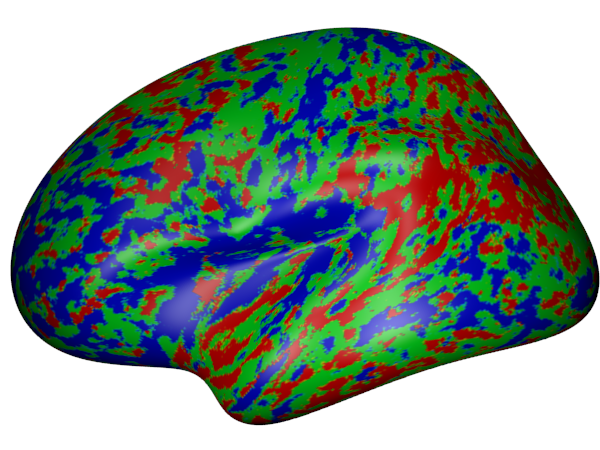
\includegraphics[scale=0.15]{slopeCol_drcThFWHM0Initk-meansCl3Pr0Ra1Mrf5_VWDPMMeanAD.png}
%  \caption{Without MRF}
%  \end{subfigure}
%  \begin{subfigure}{0.3\textwidth}
%  \centering
%  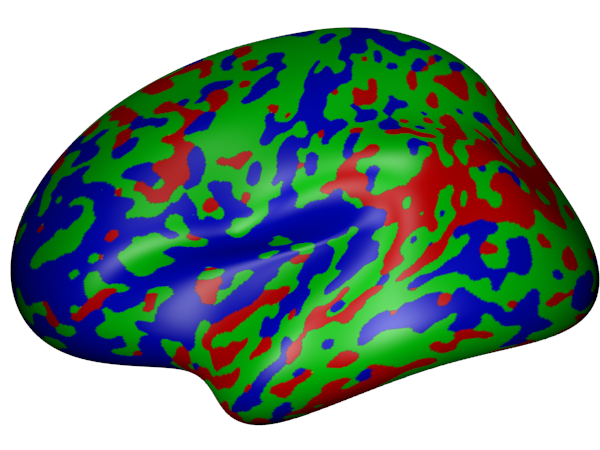
\includegraphics[scale=0.15]{slopeCol_drcThFWHM0Initk-meansCl3Pr0Ra1Mrf5_VDPM_MRFAD.png}
%  \caption{With MRF,  $\alpha = 5$.}
%  \end{subfigure}
% \end{figure}
% 
% 
% 
% \end{frame}
% 
% 
% 
% \begin{frame}[label=current]
% \frametitle{Model Fitting with Expectation-Maximisation (EM)}
% 
% % \newcommand{\mycirc}[2]{\draw (#1,#2) circle (3cm);}
% 
% % \newcommand{\outFolder}{.}
% % \small{
%     \vspace{-4em}
%     \begin{itemize}
%     \item \textbf{E-step}:
%     \begin{itemize}
%     \item Estimate vertex assignment to clusters $z_{lk}^{(u)} = \zeta_{lk}(\lambda^{(u)})$:
%      
%     $$ \lambda^{(u)} = \argmax_{\lambda}\ \sum_{l=1}^L \sum_{k=1}^K \zeta_{lk}(\lambda) \left[  D_{lk} \  + \lambda \sum_{l_2 \in N_l}  \zeta_{l_2 k}(\lambda)\  -\lambda^2 \sum_{l_2 \in N_l} (1- \zeta_{l_2 k}(\lambda))  \right]$$\\
%     $$    \zeta_{lk}(\lambda) \approx exp \left( D_{lk} +   \sum_{l_2 \in N_l} log\ \left[ exp(-\lambda^2) + z_{l_2k}^{(u-1)} (exp(\lambda) - exp(-\lambda^2)) \right] \right) $$
%     where:
%     $$ D_{lk} = -\frac{1}{2}log\ (2 \pi \left(\sigma_k^{(u)}\right)^2) |I| - \frac{1}{2\left(\sigma_k^{(u)}\right)^2} \sum_{i,j \in I} (V_l^{ij} - f(\alpha_i^{(u)} t_{ij} + \beta_i^{(u)} | \theta_k^{(u)}))^2$$
%         
%     \end{itemize}
%     \item \textbf{M-step}:
%     \begin{itemize}
%      \item Update trajectories:
%      
%      \begin{equation}
%  \label{eq:theta}
%  \theta_k = \argmin_{\theta_k} \left[\sum_{l=1}^L z_{lk} \sum_{(i,j) \in I} (V_l^{ij} - f(\alpha_i t_{ij} + \beta_i | \theta_k))^2 \right] - log\ p(\theta_k) 
% \end{equation}
%      
%      \item Update subject progression scores:
%      
%      \begin{equation}
% \label{eq:alpha}
%  \alpha_i, \beta_i = \argmin_{\alpha_i, \beta_i}  \left[ \sum_{l=1}^L \sum_{k=1}^K z_{lk} \frac{1}{2\sigma_k^2} \sum_{j \in I_i} (V_l^{ij} - f(\alpha_i t_{ij} + \beta_i | \theta_k))^2\right] - log\ p(\alpha_i, \beta_i)
% \end{equation}
%      
%     \end{itemize}
%     \end{itemize}
% \vspace{-3em}
%     
% \end{frame}


\end{document}



